\documentclass{article}
\author{Austin Hall}
\date{March 2020}
\title{\huge Capacitative Rain Gauge}
\usepackage{natbib}
\usepackage{graphicx}
\usepackage{amsmath}
\usepackage{epstopdf}

\begin{document}
\maketitle
\begin{center}
{\LARGE Abstract}\\
\end{center}

\newpage
\section{Introduction}


\newpage
\section{Theory and Methods}


\newpage
\section{Results}
\begin{figure}[h!]
\centering
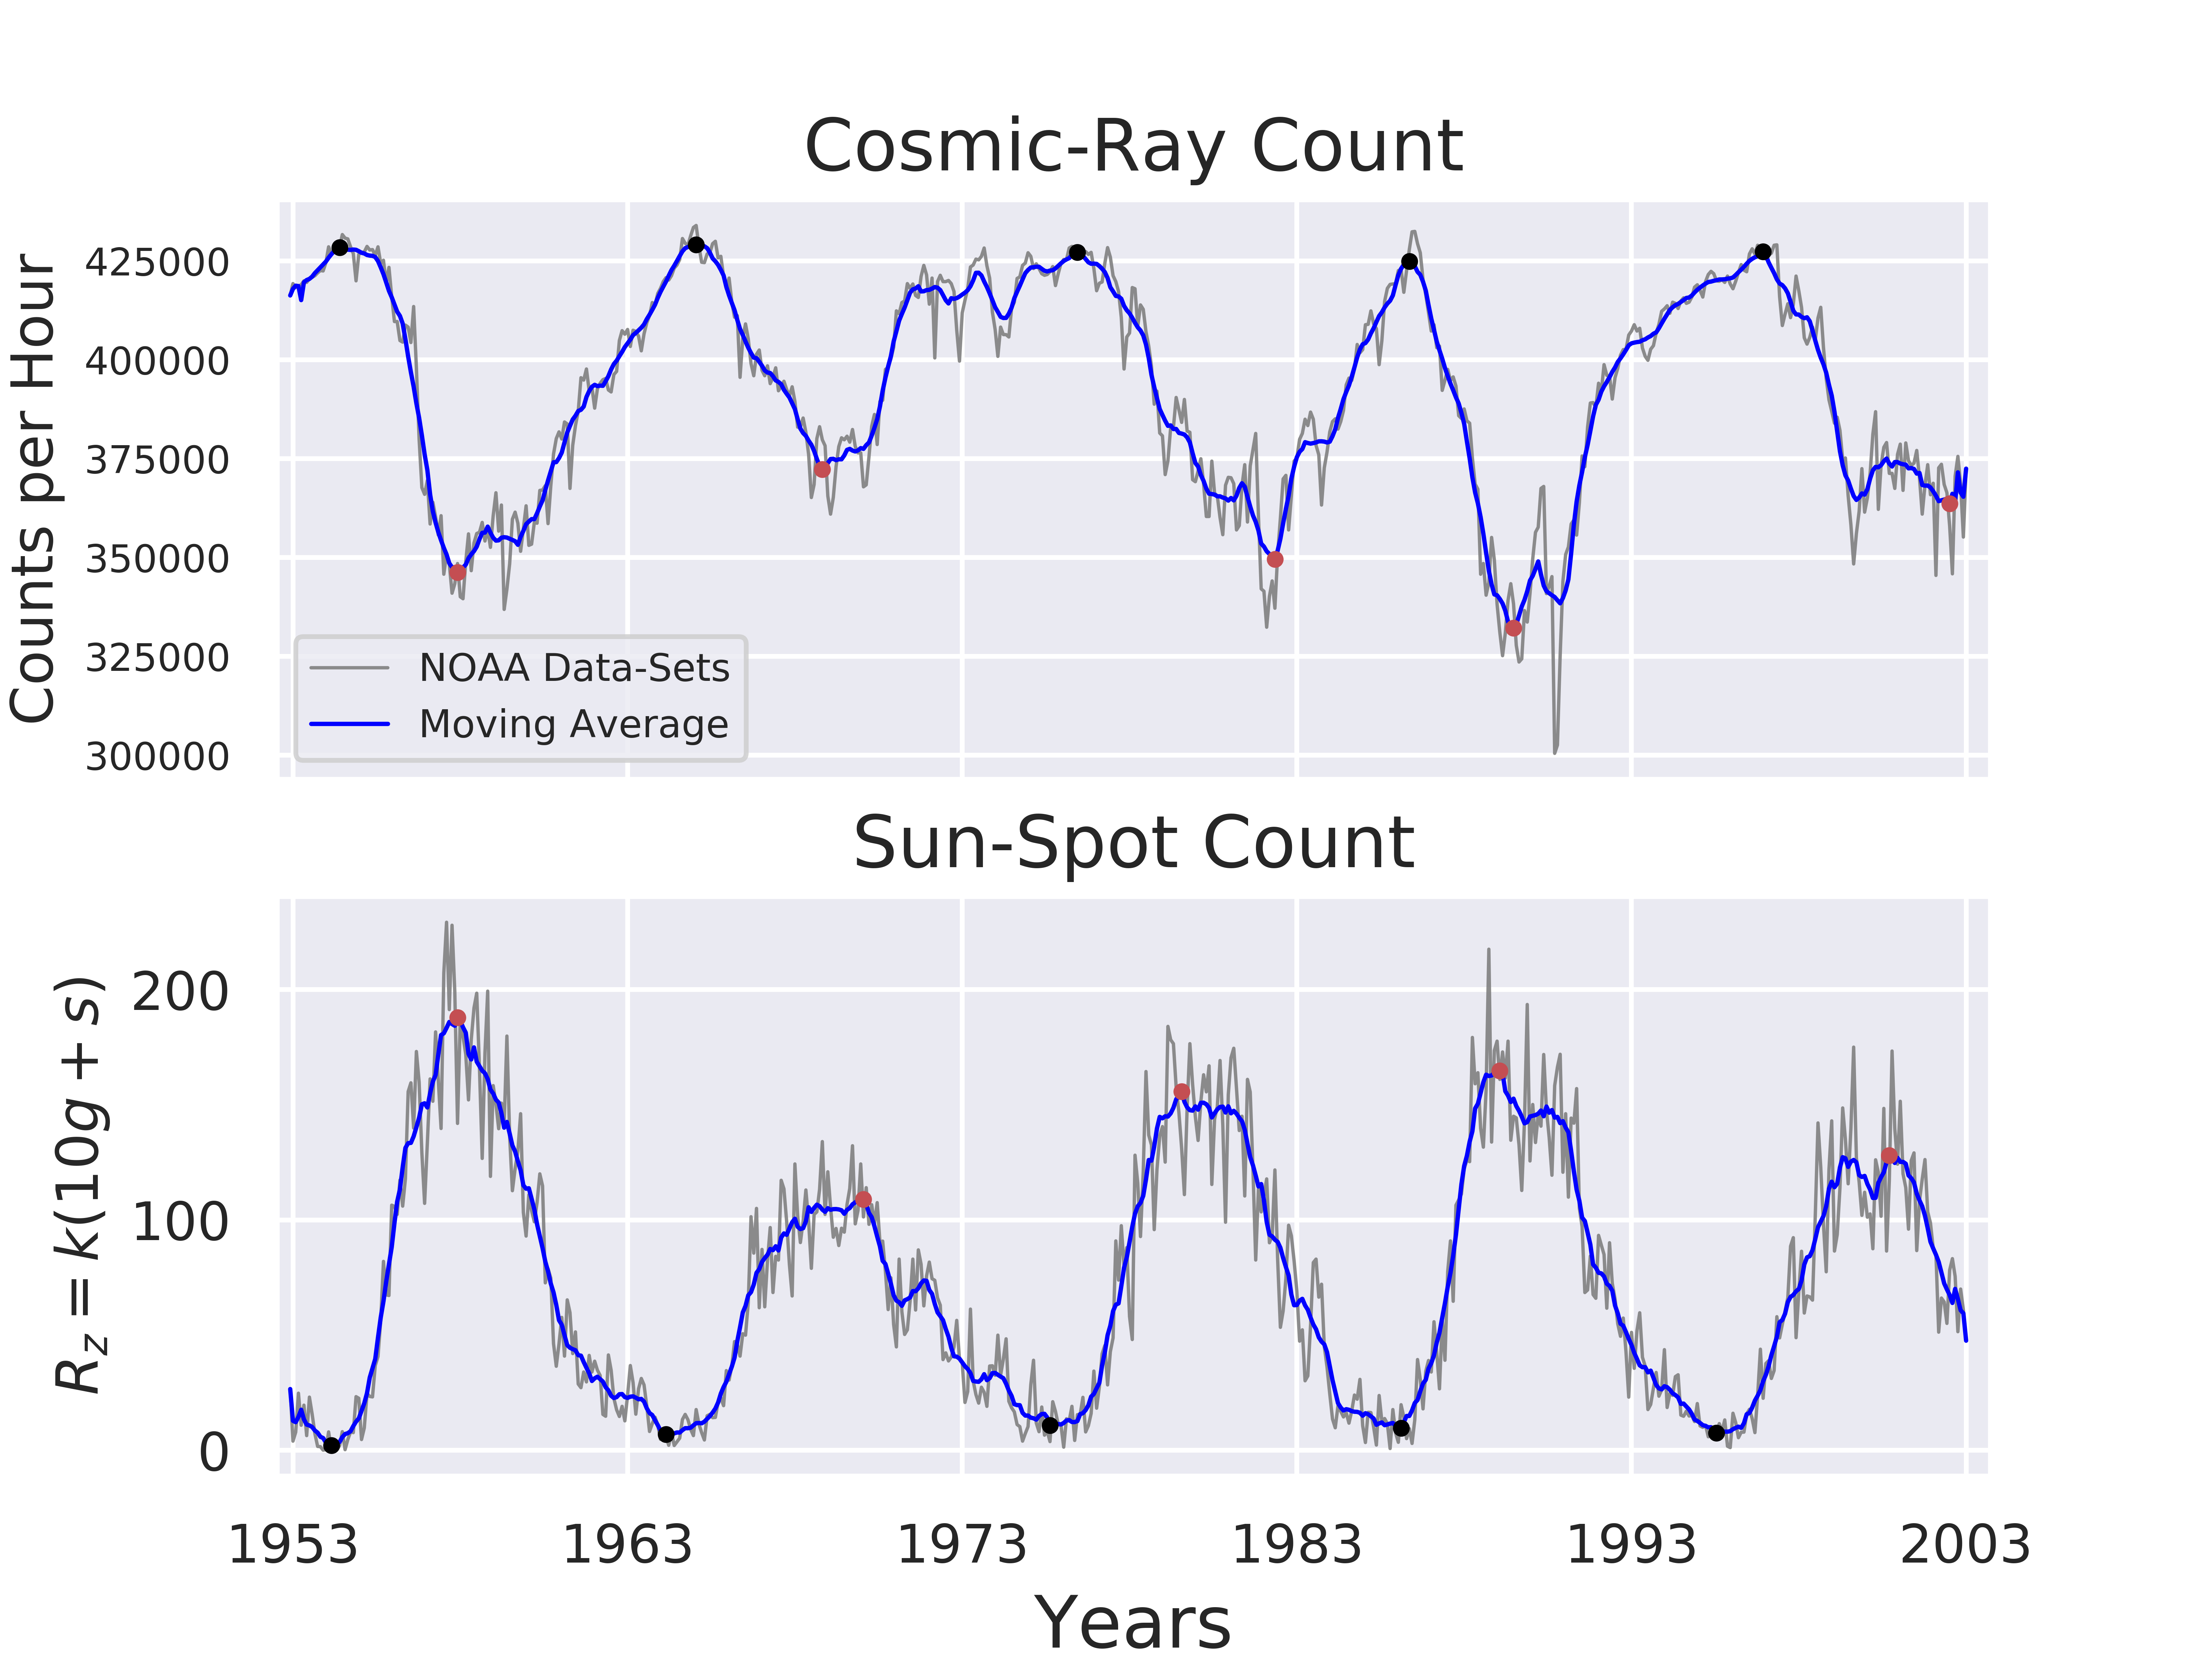
\includegraphics[scale=0.35]{plot.png}
\caption{Results Obtained with Python}
\label{fig:SunData}
\end{figure}

\newpage
\section{Analysis}


\newpage
\section{Conclusion}
\newpage
\bibliographystyle{plain}

\end{document}
